\documentclass[aspectratio=169]{beamer}

\usetheme{default}
\usecolortheme{default}
\setbeamertemplate{navigation symbols}{}
\setbeamertemplate{footline}[frame number]

\usepackage{graphicx}
\usepackage{booktabs}
\usepackage{tikz}
\usetikzlibrary{shapes.geometric, arrows, positioning}

% Define colors
\definecolor{darkblue}{RGB}{0,51,102}
\definecolor{lightblue}{RGB}{51,102,153}

% Set fonts
\setbeamerfont{title}{size=\LARGE, series=\bfseries}
\setbeamerfont{frametitle}{size=\Large, series=\bfseries}
\setbeamercolor{frametitle}{fg=darkblue}

\title{Weekly NFL Fantasy Football Point Forecasting\\Using Gradient Boosting Models}
\author{Steven DeFalco, Liam Guske, Nick Obiso}
\institute{Stevens Institute of Technology\\AAI 595 Applied Machine Learning}
\date{}

\begin{document}

% Slide 1: Title & Context
\begin{frame}
\titlepage
\vspace{-1em}
\begin{center}
\large
Predicting weekly fantasy points using machine learning\\
on NFL play-by-play data (2009--2016)
\end{center}
\end{frame}

% Slide 2: Why Weekly Fantasy Forecasting Is Hard
\begin{frame}
\frametitle{Why Weekly Fantasy Forecasting Is Hard}
\vspace{1em}
\large
\begin{itemize}
\setlength\itemsep{1.5em}
\item \textbf{High week-to-week variance:} Individual game outcomes are noisy and unpredictable
\vspace{0.5em}
\item \textbf{Context-dependent performance:} Opponent matchups, injuries, weather, and game script matter
\vspace{0.5em}
\item \textbf{Limited historical data:} Only 16--17 games per season per player
\end{itemize}
\vspace{1em}
\begin{center}
\large
$\Rightarrow$ Need time-aware ML models, not just season-long averages
\end{center}
\end{frame}

% Slide 3: Data & Pipeline Overview
\begin{frame}
\frametitle{Data \& Pipeline Overview}
\vspace{0.5em}
\begin{center}
\large
\textbf{Data Processing Pipeline}
\vspace{0.5em}

\begin{columns}[c]
\begin{column}{0.20\textwidth}
\centering
\fcolorbox{black}{lightblue!20}{\parbox{0.9\textwidth}{\centering\scriptsize Play-by-Play\\Data}}
\end{column}
\begin{column}{0.05\textwidth}
\centering
\Large $\rightarrow$
\end{column}
\begin{column}{0.20\textwidth}
\centering
\fcolorbox{black}{lightblue!20}{\parbox{0.9\textwidth}{\centering\scriptsize Player-Week\\Aggregates}}
\end{column}
\begin{column}{0.05\textwidth}
\centering
\Large $\rightarrow$
\end{column}
\begin{column}{0.20\textwidth}
\centering
\fcolorbox{black}{lightblue!20}{\parbox{0.9\textwidth}{\centering\scriptsize Feature\\Engineering}}
\end{column}
\begin{column}{0.05\textwidth}
\centering
\Large $\rightarrow$
\end{column}
\begin{column}{0.20\textwidth}
\centering
\fcolorbox{black}{lightblue!20}{\parbox{0.9\textwidth}{\centering\scriptsize Predictions}}
\end{column}
\end{columns}
\end{center}

\vspace{1.5em}
\Large
\begin{itemize}
\setlength\itemsep{0.7em}
\item \textbf{Seasons:} 2009--2016 (8 years)
\item \textbf{Player-weeks:} $\sim$40,000 observations
\item \textbf{Features:} 51 time-aware features (lag, rolling, season-to-date)
\item \textbf{Scoring:} Half-PPR computed directly from play-by-play
\end{itemize}
\end{frame}

% Slide 4: Methodology
\begin{frame}
\frametitle{Methodology: Features, Split, Baselines}
\vspace{0.5em}

\begin{columns}[T]
\begin{column}{0.48\textwidth}
\Large
\textbf{Feature Types:}
\large
\begin{itemize}
\setlength\itemsep{0.8em}
\item Lag variables (previous week)
\item Rolling averages (3, 5, 8 weeks)
\item Season-to-date aggregates
\item Trend indicators
\item Usage metrics
\end{itemize}
\vspace{0.5em}
\Large
\textbf{Strict historical-only:}\\
\large No current-week leakage
\end{column}

\begin{column}{0.48\textwidth}
\Large
\textbf{Time-Based Split:}
\begin{center}
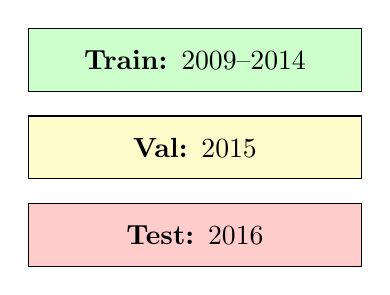
\begin{tikzpicture}[node distance=0.3cm,
    box/.style={rectangle, draw, text width=4cm, text centered, minimum height=0.8cm, font=\normalsize}]
    
\node [box, fill=green!20] (train) {\textbf{Train:} 2009--2014};
\node [box, fill=yellow!20, below=of train] (val) {\textbf{Val:} 2015};
\node [box, fill=red!20, below=of val] (test) {\textbf{Test:} 2016};
\end{tikzpicture}
\end{center}

\vspace{1em}
\Large
\textbf{Baselines:}
\large
\begin{itemize}
\item Last week
\item 3-week rolling avg
\item 5-week rolling avg
\end{itemize}
\end{column}
\end{columns}
\end{frame}

% Slide 5: Results - Model Comparison
\begin{frame}
\frametitle{Results: Model Comparison}
\vspace{-0.3em}
\begin{center}
\includegraphics[height=0.55\textheight]{../artifacts/visuals/baseline_vs_models_mae.png}
\end{center}

\vspace{0.5em}
\Large
\begin{itemize}
\setlength\itemsep{0.5em}
\item \textbf{Best Model:} Histogram Gradient Boosting
\item \textbf{Test MAE:} 2.62 fantasy points
\item \textbf{Improvement:} 45\% better than best baseline (5-week rolling: 4.76)
\item \textbf{R² Score:} 0.726 (explains 72.6\% of variance)
\end{itemize}
\end{frame}

% Slide 6: What the Model Learned
\begin{frame}
\frametitle{What the Model Learned: Feature Importance}
\vspace{-0.3em}
\begin{center}
\includegraphics[height=0.6\textheight]{../artifacts/visuals/feature_importance_gb.png}
\end{center}

\vspace{0.3em}
\Large
\textbf{Key insight:} Recent form (rolling averages) dominates—sustained trends beat single-week spikes
\end{frame}

% Slide 7: Player-Level Example
\begin{frame}
\frametitle{Player-Level Example: Aaron Rodgers (2016)}
\vspace{-0.2em}
\begin{center}
\includegraphics[height=0.65\textheight]{../artifacts/visuals/player_arodgers_pred_vs_actual.png}
\end{center}

\vspace{0.5em}
\large
Model tracks trends well but struggles with extreme outliers
\end{frame}

% Slide 8: Limitations & Wrap-Up
\begin{frame}
\frametitle{Limitations \& Future Work}
\vspace{1em}
\Large

\textbf{What this system is good for:}
\begin{itemize}
\setlength\itemsep{0.8em}
\item Weekly lineup decisions based on recent trends
\item Outperforming naive heuristics in realistic forecasting scenarios
\end{itemize}

\vspace{1.5em}
\textbf{Limitations \& Next Steps:}
\begin{itemize}
\setlength\itemsep{0.8em}
\item Does not capture contextual factors (opponent strength, injuries, weather)
\item Missing Week 1 data limits early-season predictions
\item Future: Incorporate matchup features, ensemble predictions, multi-step forecasting
\end{itemize}

\vspace{1.5em}
\begin{center}
\LARGE
\textbf{Questions?}
\end{center}
\end{frame}

\end{document}
